\section{Per-Cube Surface Extraction}
\label{sec:percube}

\plain{In brief: the completed prediction is a slab of lit voxels, several voxels thick, not a surface. This stage turns each cube of it into a thin, consistently oriented, single-sided triangle mesh --- and, more importantly, declines to connect anything it cannot justify. Every operation here is local, so that neighbouring cubes independently produce matching geometry along their shared border.}

This is where the volume becomes geometry. Its outputs serve three consumers: verified local patches, cube-level inspection, and --- for the active whole-sheet path --- the pre-weld mesh pile consumed directly by the ribbon fit of Section~\ref{sec:quadribbon}. The operations below generate \emph{local surface evidence}. They do not establish large-scale wrap identity, and in particular the fact that two fronts can be connected is not treated as evidence that they should be.

\begin{figure*}[t]
  \centering
  \begin{subfigure}[b]{0.24\linewidth}
    \centering
    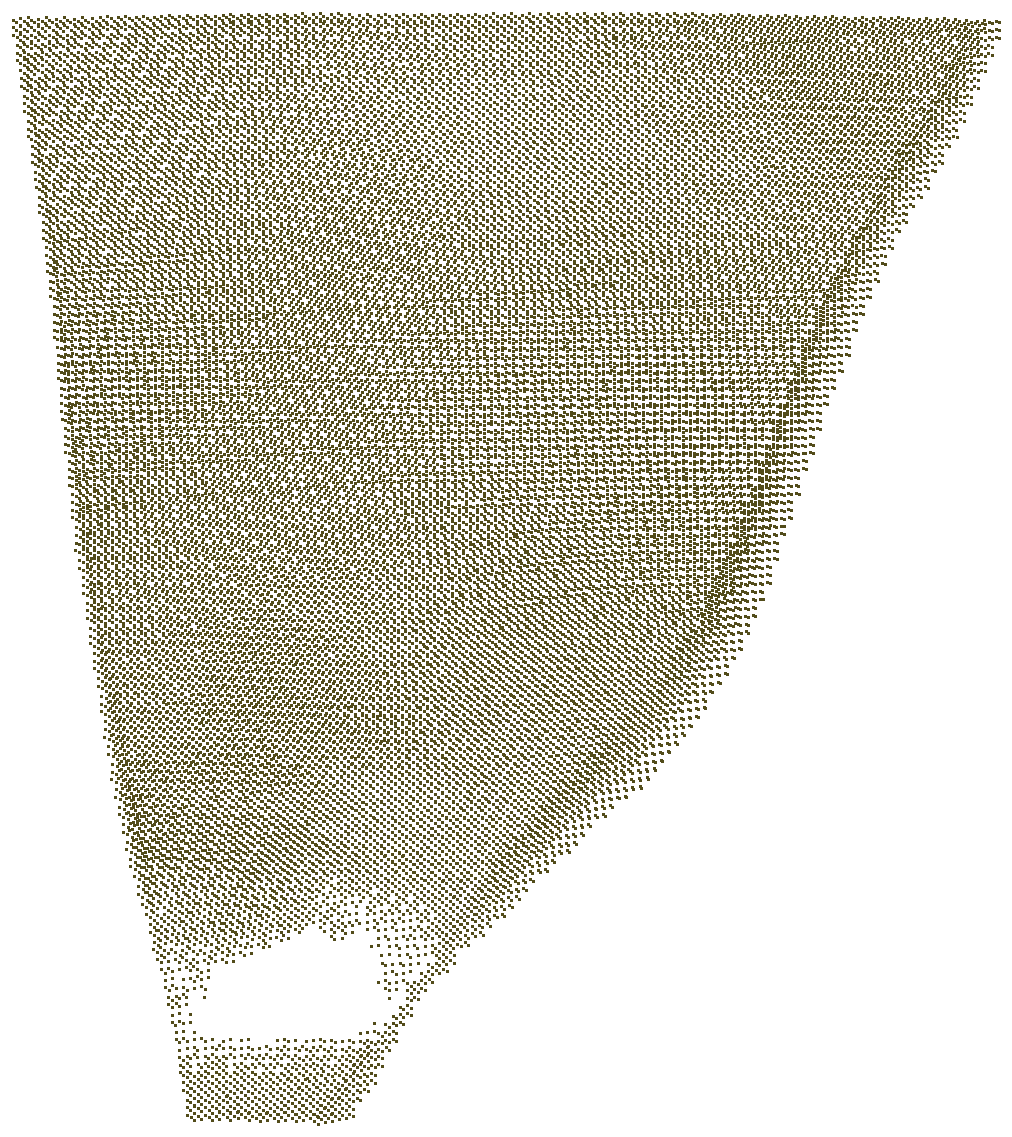
\includegraphics[width=\linewidth]{figures/overview00_crop.png}
    \caption{MLS-collapsed points}
  \end{subfigure}
  \hfill
  \begin{subfigure}[b]{0.24\linewidth}
    \centering
    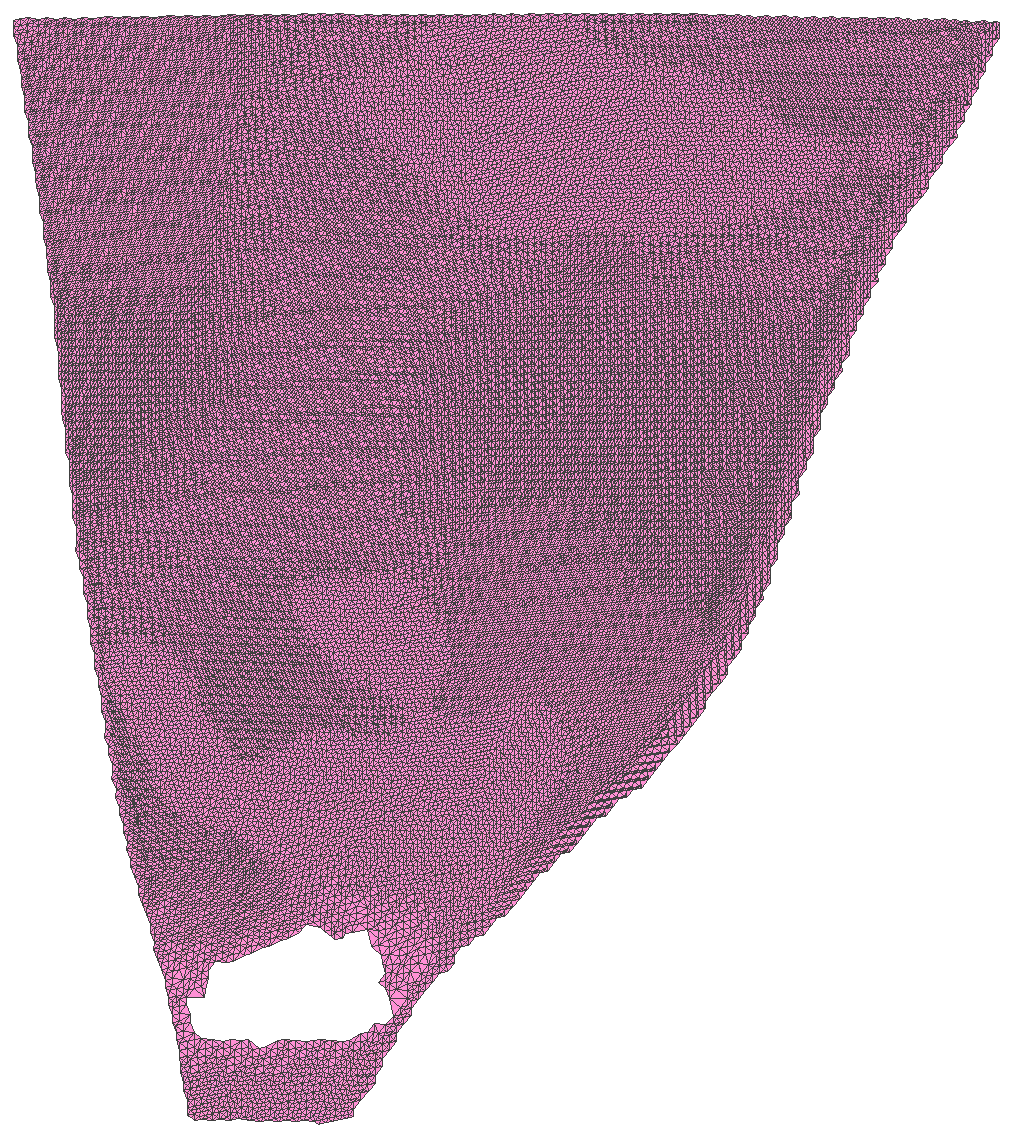
\includegraphics[width=\linewidth]{figures/overview01_crop.png}
    \caption{Guarded ball pivoting}
  \end{subfigure}
  \hfill
  \begin{subfigure}[b]{0.24\linewidth}
    \centering
    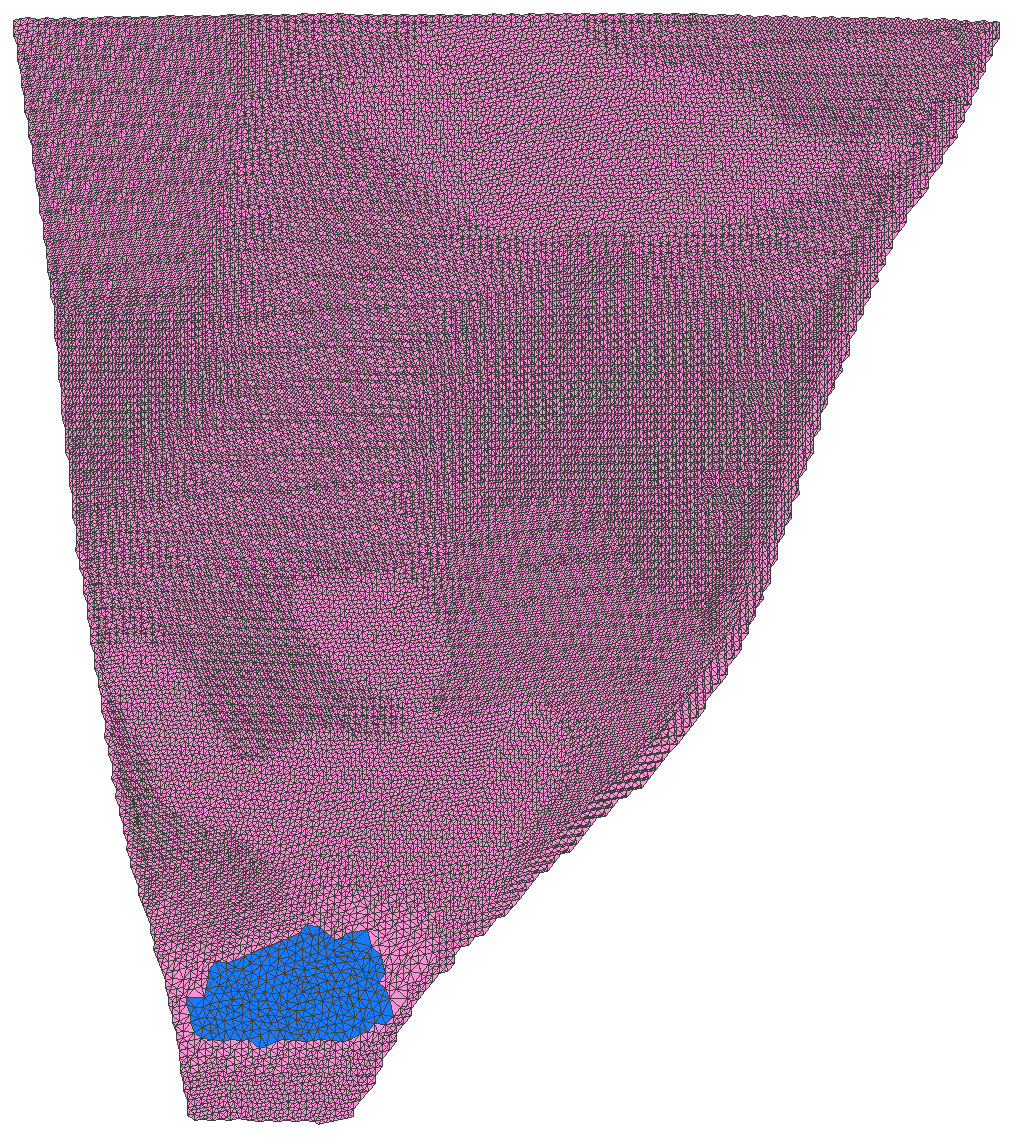
\includegraphics[width=\linewidth]{figures/overview02_crop.png}
    \caption{Interior loops filled (blue)}
  \end{subfigure}
  \hfill
  \begin{subfigure}[b]{0.24\linewidth}
    \centering
    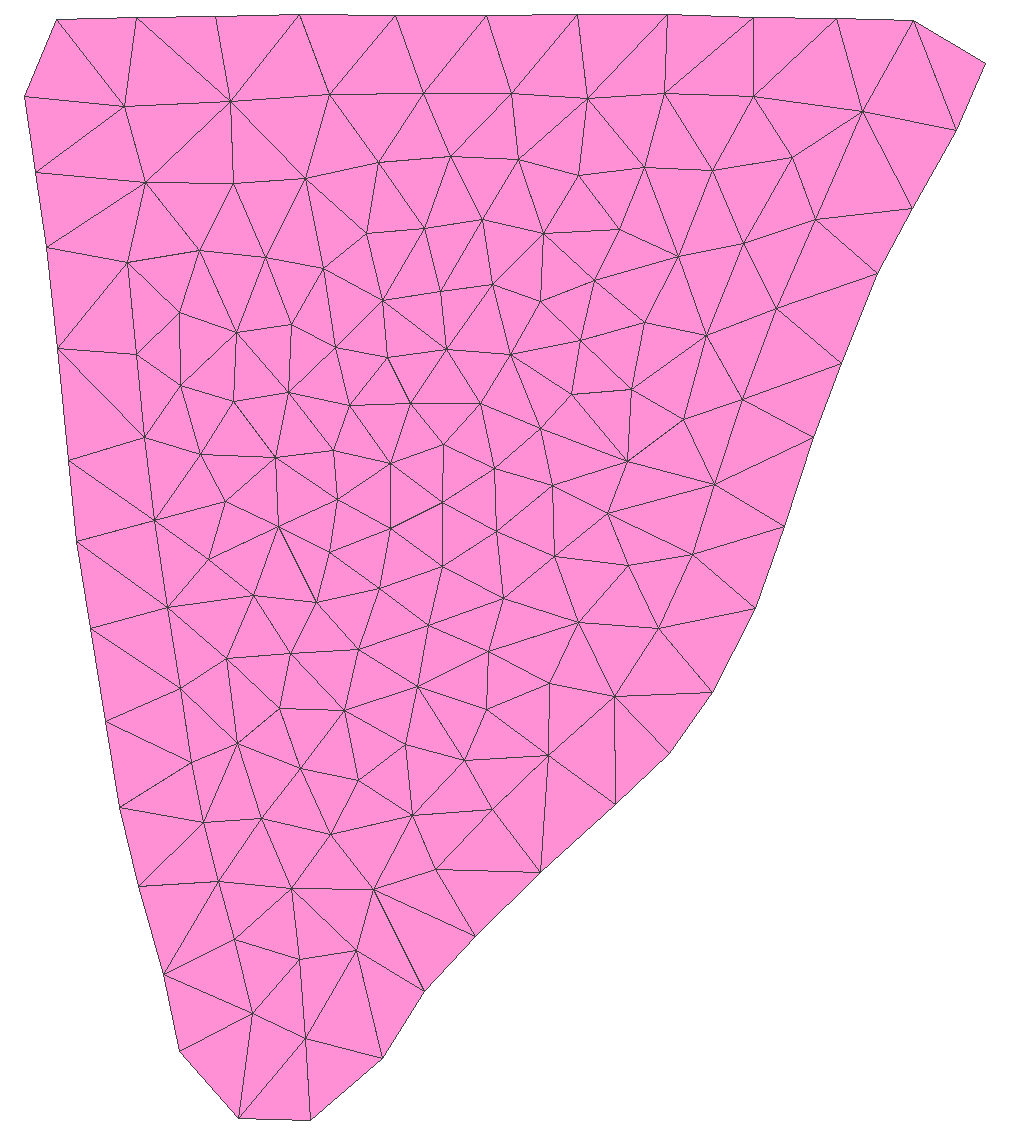
\includegraphics[width=\linewidth]{figures/overview03_crop.png}
    \caption{CVT/RVD remesh}
  \end{subfigure}
  \caption{The per-cube extraction stages on one PHerc0139 sheet. (a) Voxel-centre points after the iterated MLS projection has collapsed the several-voxel-thick prediction to a single sheet. (b) The consistently oriented, guarded ball-pivoting reconstruction; the remaining perforations are prediction gaps, not meshing failures. (c) Clean interior loops are closed (filled regions in blue) while the genuine sheet boundary is left open. (d) The level-of-detail stage on the same sheet: the CVT/RVD remeshing of Section~\ref{sec:cvt} relocates samples into a near-isotropic blue-noise distribution.}
  \Description{Four panels showing the same roughly triangular papyrus sheet as a dotted point cloud, a dense pink triangle mesh with holes, the same mesh with blue filled patches, and a coarse triangulated version.}
  \label{fig:cube_stages}
\end{figure*}

\subsection{Input Guard}

Before meshing a cube we apply a lightweight input guard. A U-Net occasionally emits a degenerate prediction in which a region is filled as a solid block rather than a thin sheet. Ball pivoting cannot roll across a solid three-dimensional point fill, and meshing such a cube yields only fragmented debris that pollutes everything downstream. We detect these cubes by morphological erosion-survival: a small 3-D erosion dissolves a genuine thin sheet entirely, while a solid slab retains a large interior fraction. We additionally require that the surviving foreground form a solid filled rectangle across many consecutive slices, so that dense but legitimate wrap regions --- which are thin sheets pressed close together, not slabs --- are never rejected. A cube failing this guard is skipped and contributes nothing, rather than contributing junk.

\subsection{Collapse to a Single Sheet}

We initialize the point cloud by taking one point at the centre of each solid voxel of the input cube. Where the prediction is more than one voxel thick this yields a slab of points several voxels deep, so we first collapse and denoise it into a single clean sheet using an iterated moving least-squares (MLS) projection~\cite{levin2003mesh}: each point is moved along its local surface normal, estimated from a Wendland-weighted neighbourhood~\cite{wendland1995piecewise}, onto the local least-squares plane. Only the through-thickness component of this motion is non-zero, so the slab is thinned without the in-plane contraction we observed when we initially tried the closely related locally optimal projection~\cite{lipman2007parameterization}.

The projection itself is a standard tool. Our observation is that choosing a projection whose kernel has \emph{compact support} makes the per-cube result consistent across cube boundaries, and that this boundary-consistency is precisely what makes divide-and-conquer scroll meshing possible at all. Concretely, adjacent cubes are processed with an overlapping halo of shared input voxels; because each projected position depends only on neighbours within a fixed radius, points in the shared region land in the same place in both cubes, and the two cubes therefore present matching geometry to whatever composes them. Finally, we trim the cloud so that the open mesh boundary falls inside the cube face, and weld points lying within 0.25 voxels of one another.

We then assign the point cloud a globally consistent normal orientation using the method of Hoppe et al.~\shortcite{hoppe1992surface}, so that all papyrus surfaces are consistently oriented as the rest of the pipeline requires.

\subsection{Guarded Ball Pivoting}
\label{sec:bpa}

Meshing the point cloud requires an algorithm that is local (so cubes can be joined afterwards), fast, and --- critically --- not designed to output a closed watertight surface. We therefore use the ball-pivoting algorithm~\cite{bernardini1999ball} (BPA): three points form a triangle if a ball of user-specified radius $\rho$ touches them without containing any other point; starting from a seed triangle, the ball pivots around each edge until it touches another point, forming the next triangle, and the process continues until all reachable edges have been tried, then restarts from a new seed. This satisfies our criteria at the cost of some small topological artifacts that are straightforwardly repaired (Section~\ref{sec:cleanup}). It also composes: cube surfaces can be joined by setting the cube boundaries to the advancing front at start-up, and it is very well behaved on open surfaces.

The unguarded algorithm, however, has exactly the failure mode this problem cannot tolerate: given two sheets 7 voxels apart and a ball of radius 1.2, a front that reaches the edge of its own sheet will happily roll down onto the neighbour. Our implementation therefore carries five guards, each aimed at a specific mechanism.

\begin{itemize}
  \setlength{\itemsep}{2pt}
  \item A \textbf{dihedral fold-back guard} prevents the front from folding back over itself.
  \item A \textbf{face-coherence guard} rejects any candidate triangle whose normal turns too sharply away from the triangle owning the pivot edge. Without it, the ball tends to roll onto an adjacent wrap instead of across a thin gap in its own sheet, stitching the two layers together.
  \item An \textbf{anti-parallel guard} refuses a triangle that would bridge two oppositely oriented surfaces lying close together, as occurs wherever neighbouring wraps nearly touch.
  \item A \textbf{wall guard} rejects candidates that are simultaneously steep against the local MLS normal \emph{and} long. A fusion bridge stands nearly perpendicular to the sheet it fuses and must reach across the inter-wrap gap, whereas a genuine surface triangle lies parallel to its vertex normals; the conjunction of the two conditions fires on through-thickness bridges and spares sharp folds.
  \item A \textbf{winding growth guard} addresses the gradual failure. Because a front can accumulate error slowly --- every individual pivot innocent while the front climbs a through-thickness wall and gains whole turns --- each seed carries the branch-cut-free integrated winding phase of Equation~\eqref{eq:winding} along its growth, and a pivot whose accumulated phase leaves a tolerance band is rejected. The surface beyond it is re-seeded as a distinct component rather than silently attached.
\end{itemize}

Guard thresholds appear in Appendix~\ref{app:terms}, each with the measurement that fixed it.

\paragraph{Adaptive radius selection.} A smaller pivot radius can sometimes avoid a local fusion, but it can also discard surface coverage and explode the number of open boundary edges, so $\rho$ is not tuned by appearance. The controller begins at the nominal radius and tries smaller radii only after a winding failure. A candidate is accepted when it contains no abrupt full-turn edges or broad branch-local fusions, retains at least 95\% of the baseline point coverage, and introduces no more than $1.25\times$ the baseline boundary edges --- a three-way trade between fusion, coverage, and boundary complexity that a single radius cannot resolve for every cube. If no candidate satisfies all three, the component is set aside for cutting rather than meshed at a radius known to fuse it.

\subsection{Topological Cleanup}
\label{sec:cleanup}

\plain{In brief: four repairs, in a fixed order, each removing a defect that would otherwise be indistinguishable from real structure later on.}

\paragraph{Separate, then re-project.} A single voxel connected-component can hold several \emph{disconnected} surface sheets that were projected and meshed together, because the MLS projection operates on all of a component's points at once and nearby sheets pull on one another. Before anything else, we separate each meshed component into its connected pieces and re-project and re-mesh each one in isolation --- this time from its \emph{original} voxel-centre points rather than from the already-projected vertices, so that the projection kernel sees only same-sheet neighbours and each sheet lands cleanly on its own surface. Re-projecting from the original points proves to be a reusable primitive; we apply it after every split below, to clean the ragged boundary a cut otherwise leaves behind.

\paragraph{Sever fused components.} Multiple components may still be erroneously attached within one cube, either through proximity during ball pivoting or, more commonly, through errors in the input prediction. Now that we have meshes, we can detect these connections: we find every connected mesh component in the cube and cast rays from each triangle centroid along its normal in both directions to determine whether the geometry should be split.

We categorize splits into two cases. Where one small bridge connects two levels of geometry --- commonly caused by segmenter artifacts (Fig.~\ref{fig:bridgesplit}a,b) --- we formulate the split as a min-cut problem solved by Edmonds--Karp. For more complex overlapping geometries we use a lifted multicut solver~\cite{keuper2015efficient} on an overlap-reduction problem in the formulation of Limper et al.~\cite{limper2018box}. After splitting, each resulting piece is re-projected and re-meshed from its parent's original voxel points, so the new sheet boundaries come out clean rather than carrying the jagged trace of the cut.

\begin{figure*}[t]
  \centering
  \begin{subfigure}[b]{0.245\linewidth}
    \centering
    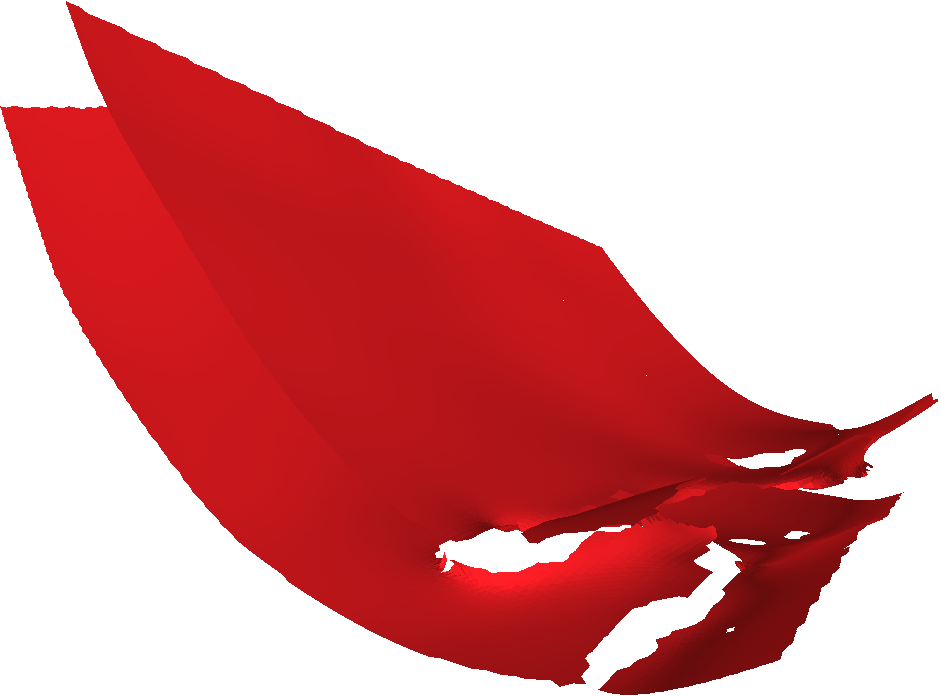
\includegraphics[width=\linewidth]{figures/neck_before00.png}
    \caption{Fused pair, before}
    \label{fig:bridgesplit_before}
  \end{subfigure}
  \hfill
  \begin{subfigure}[b]{0.245\linewidth}
    \centering
    
\includegraphics[width=\linewidth]{figures/neck_after01.png}
    \caption{Severed at the neck}
    \label{fig:bridgesplit_after}
  \end{subfigure}
  \hfill
  \begin{subfigure}[b]{0.245\linewidth}
    \centering
    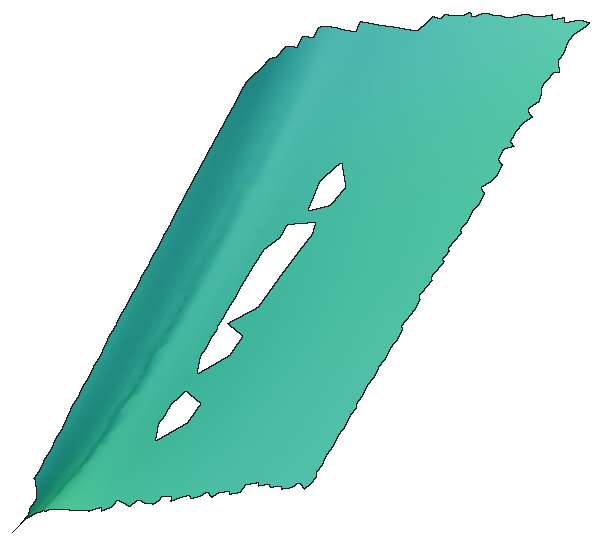
\includegraphics[width=\linewidth]{figures/holefill_before.png}
    \caption{Perforated sheet, before}
    \label{fig:holefill_before}
  \end{subfigure}
  \hfill
  \begin{subfigure}[b]{0.245\linewidth}
    \centering
    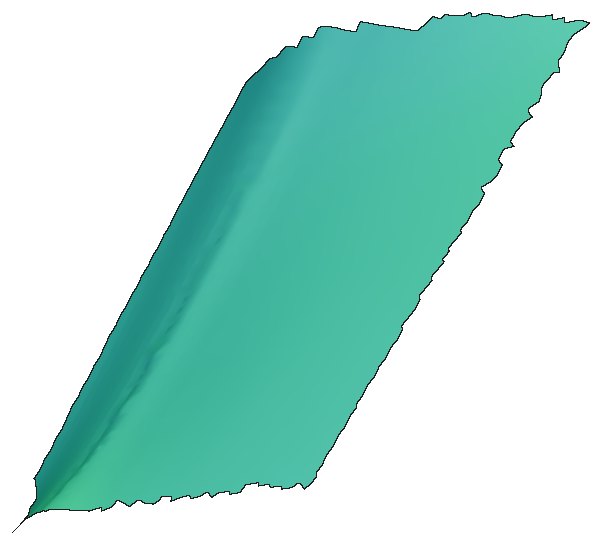
\includegraphics[width=\linewidth]{figures/holefill_after.png}
    \caption{Interior loops closed}
    \label{fig:holefill_after}
  \end{subfigure}
  \caption{The two mesh-space repairs that must happen before any parameterization is attempted, on real PHerc0139 cubes. (a,b) The U-Net has fused two sheets through a thin neck of bridge material; the bridge is detected and severed by min-cut, recovering two distinct sheets. A fusion left in place would weld two wraps into one and make the winding topology unrecoverable --- and, per Section~\ref{sec:gp}, nothing further downstream could tell. (c,d) Holes left by the ball-pivoting front and by gaps in the prediction are closed: exact three-edge loops directly, larger clean interior loops by constrained Delaunay with Liepa-style refinement~\cite{liepa2003filling}. Self-intersecting, non-manifold, or clearly exterior loops are rejected rather than force-filled, so a genuine sheet boundary is never sealed shut.}
  \Description{Four small panels: two mesh sheets joined by a thin bridge and then separated at it, followed by a perforated triangle mesh and the same mesh with its interior holes closed.}
  \label{fig:bridgesplit}
\end{figure*}

\paragraph{Close interior holes.} After each separation we split pinched vertex fans until every component is vertex-manifold. Holes detected inside a component are then patched (Fig.~\ref{fig:bridgesplit}c,d): exact three-edge loops are closed directly, and other clean interior loops are projected to a local plane, triangulated by constrained Delaunay, and lifted back with Liepa-style refinement~\cite{liepa2003filling}. Self-intersecting, non-manifold, or clearly exterior loops are rejected rather than force-filled --- the distinction matters because sealing a genuine torn edge would convert a known boundary into fabricated papyrus.

\paragraph{Open accidental handles.} Ball pivoting can also fuse a sheet to itself \emph{without} disconnecting it: where the advancing front rolls across a thin gap, it can close a loop that raises the sheet's genus into a small handle. Such handles are \emph{non-separating}, so the cut-based splitters above, which sever \emph{separating} necks, cannot remove them. After hole filling we therefore apply a tree--cotree decomposition and open every non-separating loop shorter than a fixed length bound by manifold-preserving vertex duplication. A per-cube sheet has no legitimate scroll-scale handle, so this reduces accidental local genus while leaving the long cycles that represent genuine structure untouched.

\subsection{CVT/RVD Remeshing}
\label{sec:cvt}

Earlier versions of ScrollFiesta used quadric error metrics (QEM) to downsample the ball-pivoting output. In practice this created numerous sliver triangles and an uneven distribution of samples, both of which are poison for a later metric parameterization. We therefore perform level-of-detail with a centroidal Voronoi tessellation restricted to the reconstructed surface. We seed interior sites by area and boundary sites along every retained loop, then iterate the variational update of CWF~\cite{xu2024cwf}: each interior site solves a small fixed-cell system combining the ordinary centroidal (CVT) term with a normal-anisotropy term that pulls samples onto creases and thin features, with the CVT weight decaying across iterations (Appendix~\ref{app:cvt}). Each updated site is projected back to the source surface, and the output triangles are the restricted-Delaunay dual of the restricted Voronoi diagram (RVD). Uniform density is used per cube at present. Unlike collapse-only QEM, this relocates samples into a near-isotropic distribution, reduces slivers, and does not preserve a poor advancing-front tessellation merely because it arrived first.

One caution is worth recording, because it is a case of the failure described in Section~\ref{sec:gp}. A remesher is a purely geometric operator and has no notion of wrap identity: run with an interior edge length above the local pitch, it will happily merge turn $N$ into turn $N{+}1$, producing a perfectly clean mesh that is physically wrong. The CVT stage therefore runs under the same winding bound as the mesher, armed from the measured umbilicus and pitch, and its edge budget is bounded below the clearance rather than chosen for triangle count.

Any component above the current size cap, an empty or invalid dual, or a result failing the manifold checks falls back to the repaired QEM path, which can also be selected explicitly; that fallback rejects edge collapses or maintenance flips that would create an existing edge or reverse winding. Once remeshed, components with negligible area are removed as debris, and halo output is cut at the owned cube planes so that every geometric region has exactly one owner at assembly time.
